\documentclass[apacite,linguex]{glossa}\usepackage[]{graphicx}\usepackage[]{color}
% maxwidth is the original width if it is less than linewidth
% otherwise use linewidth (to make sure the graphics do not exceed the margin)
\makeatletter
\def\maxwidth{ %
  \ifdim\Gin@nat@width>\linewidth
    \linewidth
  \else
    \Gin@nat@width
  \fi
}
\makeatother

\definecolor{fgcolor}{rgb}{0.345, 0.345, 0.345}
\newcommand{\hlnum}[1]{\textcolor[rgb]{0.686,0.059,0.569}{#1}}%
\newcommand{\hlstr}[1]{\textcolor[rgb]{0.192,0.494,0.8}{#1}}%
\newcommand{\hlcom}[1]{\textcolor[rgb]{0.678,0.584,0.686}{\textit{#1}}}%
\newcommand{\hlopt}[1]{\textcolor[rgb]{0,0,0}{#1}}%
\newcommand{\hlstd}[1]{\textcolor[rgb]{0.345,0.345,0.345}{#1}}%
\newcommand{\hlkwa}[1]{\textcolor[rgb]{0.161,0.373,0.58}{\textbf{#1}}}%
\newcommand{\hlkwb}[1]{\textcolor[rgb]{0.69,0.353,0.396}{#1}}%
\newcommand{\hlkwc}[1]{\textcolor[rgb]{0.333,0.667,0.333}{#1}}%
\newcommand{\hlkwd}[1]{\textcolor[rgb]{0.737,0.353,0.396}{\textbf{#1}}}%
\let\hlipl\hlkwb

\usepackage{framed}
\makeatletter
\newenvironment{kframe}{%
 \def\at@end@of@kframe{}%
 \ifinner\ifhmode%
  \def\at@end@of@kframe{\end{minipage}}%
  \begin{minipage}{\columnwidth}%
 \fi\fi%
 \def\FrameCommand##1{\hskip\@totalleftmargin \hskip-\fboxsep
 \colorbox{shadecolor}{##1}\hskip-\fboxsep
     % There is no \\@totalrightmargin, so:
     \hskip-\linewidth \hskip-\@totalleftmargin \hskip\columnwidth}%
 \MakeFramed {\advance\hsize-\width
   \@totalleftmargin\z@ \linewidth\hsize
   \@setminipage}}%
 {\par\unskip\endMakeFramed%
 \at@end@of@kframe}
\makeatother

\definecolor{shadecolor}{rgb}{.97, .97, .97}
\definecolor{messagecolor}{rgb}{0, 0, 0}
\definecolor{warningcolor}{rgb}{1, 0, 1}
\definecolor{errorcolor}{rgb}{1, 0, 0}
\newenvironment{knitrout}{}{} % an empty environment to be redefined in TeX

\usepackage{alltt}

\let\B\relax
\let\T\relax
\usepackage{xyling} 
\usepackage[linguistics]{forest}


% \pdf* commands provide metadata for the PDF output. ASCII characters only!
\pdfauthor{Utku Turk and Pavel Logacev}
\pdftitle{Agreement Attraction in Turkish}
\pdfkeywords{agreement attraction, syncretism, Turkish, bayesian, replication}

\title[Agreement Attraction in Turkish]{Agreement Attraction in Turkish: The Case of Genitive Attractors\\ \bigskip \large Word count: 3303}

\newcommand{\firstauthor}{{Utku T\"urk}}
\newcommand{\firstauthorshort}{{T\"urk}}
\newcommand{\secondauthor}{{Pavel Loga\v{c}ev}}
\newcommand{\secondauthorshort}{{Loga\v{c}ev}}


\author[\firstauthorshort \& \secondauthorshort]% short form of the author names for the running header. If no short author is given, no authors print in the headers.
{%as many authors as you like, each separated by \AND.
  \spauthor{\firstauthor\\ 
  \institute{Bo\u{g}azi\c{c}i University}\\
  \small{
    \texttt{utku.turk@boun.edu.tr}}
  }
  \AND
  \spauthor{\secondauthor\\ 
  \institute{Bo\u{g}azi\c{c}i University}\\
  \small{
    \texttt{pavel.logacev@boun.edu.tr}}
  }%
}
\IfFileExists{upquote.sty}{\usepackage{upquote}}{}
\begin{document}







\sffamily
\maketitle


\begin{abstract}

Previous studies have shown that speakers may find sentences violating subject-verb agreement grammatical when the sentence contains a feature-matching noun phrase. This so-called agreement attraction effect has also been found in genitive possessive structures such as \textit{'the teacher's brother'} in Turkish (Lago et al., 2019), which is in contrast with its absence in similar constructions in English (Nicol et al., 2016). This discrepancy has been hypothesized to be a result of the association between genitive case marking and subjecthood in Turkish, but not in English. In the present research, we test an alternative explanation in which Turkish number agreement attraction effects are due to a potential confound in Lago et al.'s experiment, as a result of which subject head nouns were locally ambiguous between the possessive and the accusative case. We hypothesized that this ambiguity may have inhibited the availability of the head noun as an agreement controller as the accusative is a non-subject case in Turkish. To test this hypothesis, we conducted a speeded acceptability judgment experiment and our results suggest that case-ambiguity does not play a role in agreement attraction, and thus lends credibility to the claim that genitive noun phrases may function as attractors in Turkish due to the association between genitive case and subjecthood. %exclude


\end{abstract}

\begin{keywords}
agreement attraction; syncretism; Turkish; bayesian; replication
\end{keywords}

\rmfamily




\section{Introduction}

Speakers often fail to accurately process grammatical dependencies between different parts of a sentence \citep[e.g.,][]{GibsonThomas:1999,PhillipsEtAl:2011}. For example, in \ref{ex:pearlmutter}, the auxiliary verb \textit{were} erroneously agrees with the agreement-wise irrelevant attractor noun phrase headed by \textit{cabinets} instead of the agreement controller headed by \textit{key}. A number of previous studies in comprehension \citep{NicolEtAl:1997, PearlmutterGarnseyBock:1999, WagersEtAl:2009} showed that participants found sentences like \ref{ex:pearlmutter} acceptable more often and read them faster compared to their counterparts with a singular attractor. This phenomenon, known as \textit{agreement attraction} \citep{BockMiller:1991} has been attested in a number of languages, such as in Arabic \citep{TuckerEtAl:2015}, Armenian \citep{AvetisyanEtAl:2020}, German \citep{LagoFelser:2018}, Hindi \citep{BhatiaDillon:2020}, Serbian \citep{RisticEtAl:2016}, Slovak \citep{BadeckerKuminiak:2007}, Spanish \citep{LagoEtAl:2015}, and recently in Turkish \citep{LagoEtAl:2019}.


\ex. \label{ex:pearlmutter} * The \underline{key} to the cabinets \underline{were} rusty from many years of disuse. 


\citet{LagoEtAl:2019} demonstrated that genitive possessors (such as \textit{painters} in \textit{the painters' rival}) effect agreement attraction effects in Turkish. However, this finding appears to be at odds with \citeauthor{NicolEtAl:2016}'s (\citeyear{NicolEtAl:2016}) results, who failed to find a similar effect in English. \citet{LagoEtAl:2019} hypothesize that Turkish possessor noun phrases, unlike their English counterparts, may function as agreement attractors because Turkish genitive NPs may function as subjects of non-finite clauses in Turkish \citep{GokselKerslake:2005,Kornfilt:2011}. As a result, Turkish genitive NPs may match the subjecthood feature used in the cue-based retrieval of a verb's subject \citep{LewisVasishth:2005, WagersEtAl:2009, ArnettWagers:2017}.

In this paper, we test an alternative explanation of \citeauthor{LagoEtAl:2019}'s (\citeyear{LagoEtAl:2019}) findings which is related to an instance of local ambiguity in the experimental sentences in their experiment, as a result of which all subject head nouns were ambiguous between possessive and accusative case.


\section{Agreement Attraction in Turkish}

Turkish is an SOV word order language with overt case marking \citep{GokselKerslake:2005,Kornfilt:2011,Kornfilt:2013}. 
For example, the possessor in the Turkish construction in \ref{ex:possgenex}, which is similar to the Saxon Genitive, is marked with genitive case, while the head noun is marked with possessive case. 
Importantly, the possessive case marker coincides in form with the accusative case marker when the noun stem ends in a consonant: 
This is because in Turkish, case markers have different forms depending on whether the last sound of the stem is a vowel. In order to break up vowel-vowel clusters, Turkish uses epenthetic consonants such as \textit{s}, \textit{y}, or \textit{n}.  For example, the genitive case can surface as \textit{-nin} or as \textit{-in}, depending on the last consonant of the stem. The forms of the possessive marker and the accusative case are identical except for the epenthetic consonant. This means that they surface as \textit{-i} in consonant-ending words, but as \textit{-si} and \textit{-yi} respectively in vowel-ending words. 

\ex. \label{ex:possgenex}
\gll $[$$[$teknisyen-in$]$ e\u{g}itmen-i$]$ \\
    technician-\textsc{gen} instructor-\textsc{poss} \\
\glt `the instructor of the technician'


\citet{LagoEtAl:2019} demonstrated an agreement attraction effect in Turkish genitive-possessive constructions in a speeded acceptability judgment study with sentences like \ref{ex:lago}, in which the number of the attractor and the verb was manipulated. The resulting $2$x$2$ design, indicated by brackets and slashes in \ref{ex:lago}, consisted of two grammatical conditions, in which the verb agreed with the singular subject head noun, and two ungrammatical conditions, in which the verb carried plural agreement, and thus did not agree with the subject. In ungrammatical sentences, they found a higher percentage of \textit{acceptable} responses when the genitive attractor was plural than when it was singular, indicating agreement attraction. No such effect was found in grammatical sentences.


\ex. \label{ex:lago}
\gll Teknisyen-\{ler/\O\}-in e\u{g}itmen-i ola\u{g}an{\"u}st{\"u} h{\i}zl{\i} ko\c{s}-tu-\{lar/\O\}.\\
technician-\{\textsc{pl}/\textsc{sg}\}-\textsc{gen} instructor-\textsc{poss} extraordinarily fast run-\textsc{pst}-\{\textsc{pl}/\textsc{sg}\}\\
\glt `The technician's/technicians' instructor extraordinarily fast ran\{\textsc{pl}/\textsc{sg}\}.'


\citet{LagoEtAl:2019} hypothesized that these effects originated from how case and number information is encoded and retrieved: According to \citeauthor{LewisVasishth:2005}'s (\citeyear{LewisVasishth:2005}) cue-based retrieval model, phrases are encoded in a content-addressable memory as bundles of features called \textit{chunks} which include information like number, gender, case, and syntactic function \citep[e.g.,][]{SmithVasishth:2020}. Under \citeauthor{LagoEtAl:2019}'s (\citeyear{LagoEtAl:2019}) proposal, participants predict the number of the verb based on the noun phrases they process while reading the subject. In grammatical sentences with singular verb agreement, the number prediction and the verb number match, which causes no processing difficulty. In contrast, when participants fail to find the predicted number morphology on the verb, a memory-retrieval process is initiated. This process activates the search for a chunk matching two cues: the subjecthood feature ([+SUBJECT]) and the plural feature ([+PL]). While neither of the available noun phrases matches this specification in ungrammatical agreement attraction sentences, each of the NPs headed by \textit{technician} and \textit{instructor} matches one of these cues. While this partial match mostly results in participants finding the sentence ungrammatical, they may retrieve the attractor \textit{technicians} on some trials. \citet{LagoEtAl:2019} argue that this erroneous retrieval may be facilitated by the genitive case marking on the attractor, because genitive NPs can function as subjects of embedded clauses in Turkish. Due to the ubiquity of genitive subjects, attractors marked with genitive case are a priori likely to be agreement controllers.

However, a potential problem with the stimuli in the \citet{LagoEtAl:2019} study is that the stems of all head nouns such as \textit{e\u{g}itmen-i} (\textit{`instructor'}) in \ref{ex:lago} were consonant-ending, making their possessive forms ambiguous between possessive and accusative case due to case syncretism between them in vowel-ending stems \citep[pp. 66--67]{GokselKerslake:2005}.
%because the surface form of both, the possessive and accusative case is \textit{-i}. 
%locally
As a result, the head noun (\textit{'instructor'}) in \ref{ex:ambiguous} can be disambiguated towards possessive case as in \ref{ex:ambiguous_possessive}, or towards accusative case as in \ref{ex:ambiguous_accusative}, where the genitive-marked noun functions as an embedded subject, and the matrix subject is omitted due to pro-drop.

\ex.
\label{ex:ambiguous}
  \a. \textsc{Possessive Interpretation} \label{ex:ambiguous_possessive} \\
  \gll Teknisyen-in e\u{g}itmen-i ko\c{s}-tu.\\
       technician-\textsc{gen} instructor-\textsc{poss} run-\textsc{pst}\\
  \glt `The technician's instructor ran.'
  \b. \textsc{Accusative Interpretation} \label{ex:ambiguous_accusative}\\
  \gll Teknisyen-in e\u{g}itmen-i kov-du\u{g}-un-u g\"{o}r-d\"{u}-m.\\
  technician-\textsc{gen} instructor-\textsc{poss} fire-\textsc{nmlz}-\textsc{poss}-\textsc{acc} see-\textsc{pst}-\textsc{1sg}\\
  \glt `I saw the technician firing the fast.'


%{\color{red}
%\ex. %Ambiguous Part 
%\label{ex:ambiguous}\\
%\gll Teknisyen-in e\u{g}itmen-i ola\u{g}an{\"u}st{\"u} h{\i}zl{\i} \ldots \\
%technician-\textsc{gen} instructor-\textsc{poss} extraordinarily fast \ldots \\
%  \a. Simplex Sentence \label{ex:simplexreading} \\
%  \gll \ldots{} ko\c{s}-tu.\\
%  \ldots{} run-\textsc{pst}\\
%  \glt `The technician's instructor extraordinarily fast ran.'
%  \b. Embedded Sentence \label{ex:embeddedreading}\\
%  \gll \ldots{} kov-du\u{g}-un-u g\"{o}r-d\"{u}-m.\\
%  \ldots{} fire-\textsc{nmlz}-\textsc{poss}-\textsc{acc} see-\textsc{pst}-\textsc{1sg}\\
%  \glt `I saw the technician firing the instructor really fast.'
%}


Because accusative NPs cannot function as subjects in Turkish, it is possible that Lago et al.'s finding of agreement attraction effects in sentences like \ref{ex:lago} are not due to the genitive attractors' association with subjecthood, but rather due to the head nouns' \textit{reduced association with subjecthood} due to its ambiguity.
%This ambiguity stems from the fact that the genitive case can serve as an embedded subject marker, and the accusative case can surface as \textit{-i}. 
% For example, on some trials, 
Because sentences like \ref{ex:lago} are locally ambiguous, participants may initially adopt an incorrect analysis of the genitive-possessive structure on some trials, and encode the genitive-marked first noun as the subject of an embedded verb and the ambiguous second noun as an accusative object. 
Under the assumption that remnants of an incorrect analysis affect the parsing process even after after a successful reanalysis \citep{Staub:2007}, the initial association between the genitive noun phrase and subjecthood may lead an agreement attraction effect. 
In contrast, this account predicts that the agreement attraction effect should be either significantly reduced or entirely absent when the head noun is unambiguous, as the function of the genitive noun phrase is disambiguated early, thus preventing potential digging-in effects \citep{Tabor:2004}.  
%
%the head noun will arguably not be treated as a subject until a possible reanalysis after reading the matrix verb. We expect this reduced association to be reflected as an overall decrease in accuracy in grammatical conditions. Upon reading the verb, participants will either find the sentence ungrammatical since they have expected a structure similar to \ref{ex:embeddedreading} or reanalyze the sentence and will judge the sentence according to the structure in \ref{ex:simplexreading}. Since there is no plural marker at the matrix verb, the plural on the attractor will not have an additional effect. However, in ungrammatical conditions in which the matrix verb has an overt plural marker, we expect to have an easier interference of a plural marked Genitive NP which was recently encoded as a subject and an overall decrease in the accuracy. 
%
We tested this hypothesis in a speeded-acceptability experiment with sentences similar to \citeauthor{LagoEtAl:2019}'s (\citeyear{LagoEtAl:2019}), but with unambiguously marked vowel-ending head nouns. 
%We expect that the agreement attraction effect may arise specifically on trials where participants misparse the two initial NP cases and where the sentence contains a plural attractor with a plural verb. On trials where participants misparse the two initial NP cases, but the sentence does not have a plural attractor or a plural verb, we expect overall higher errors without the specific effect of a plural attractor.
%}

\section{The Present Study}

The present study tested the predictions of the case syncretism account as an alternative explanation of the previously found agreement attraction effect in Turkish. To avoid the ambiguity present in \citet{LagoEtAl:2019}, we used vowel-ending head nouns nouns such as \textit{terzi} (\textit{`tailor'}), for which the possessive marker surfaces as \textit{-si} and is distinct from the accusative (\textit{-yi}). We hypothesized that if the morpho-phonological ambiguity was a key factor in agreement attraction in Turkish, unambiguous sentences like ours in \ref{ex:our_items} should not elicit attraction effects.

\ex. \label{ex:our_items}
  \a. * \textsc{Plural Attractor, Ungrammatical (Plural Verb)} \label{ex:expitem-plpl}\\
  \gll [Milyoner-ler-in \textbf{terzi-si}] tamamen gereksizce \textbf{kov-ul-du-lar}.\\
  millionaire-\textsc{pl}-\textsc{gen} tailor-\textsc{poss} completely without.reason fire-\textsc{pass}-\textsc{pst}-\textsc{pl}\\
  \glt `The millionaires' tailor were fired for no reason at all.'
  \b. \textsc{Plural Attractor, Grammatical (Singular Verb)} \label{ex:expitem-plsg} \\
  \gll [Milyoner-ler-in \textbf{terzi-si}] tamamen gereksizce \textbf{kov-ul-du}.\\
  millionaire-\textsc{pl}-\textsc{gen} tailor-\textsc{poss} completely without.reason fire-\textsc{pass}-\textsc{pst}\\
  \glt `The millionaires' tailor was fired for no reason at all.'
  \b. * \textsc{Singular Attractor, Ungrammatical (Plural Verb)} \label{ex:expitem-sgpl}\\
  \gll [Milyoner-in \textbf{terzi-si}] tamamen gereksizce \textbf{kov-ul-du-lar}.\\
  millionaire-\textsc{gen} tailor-\textsc{poss} completely without.reason fire-\textsc{pass}-\textsc{pst}-\textsc{pl}\\
  \glt `The millionaire's tailor were fired for no reason at all.'
  \b. \textsc{Singular Attractor Grammatical (Singular Verb)} \label{ex:expitem-sgsg}\\
  \gll [Milyoner-in \textbf{terzi-si}] tamamen gereksizce \textbf{kov-ul-du}.\\
  millionaire-\textsc{gen} tailor-\textsc{poss} completely without.reason fire-\textsc{pass}-\textsc{pst}\\
  \glt `The millionaire's tailor was fired for no reason at all.'
  

\subsection{Participants} 

We recruited 118 undergraduate students to participate in the experiment in exchange for course credit. All participants were native Turkish speakers, with an average age of 20 (range: 18 -- 32). The experiment was carried out following the principles of the Declaration of Helsinki and the regulations concerning research ethics at Bo\u{g}azi\c{c}i University. All participants provided informed consent before their participation and their identity are completely anonimized.

\subsection{Materials}

We used 40 sets of sentences like \ref{ex:our_items}, in which we manipulated (i) the number of the attractor noun and (ii) the number agreement on the verb. Plural number and plural agreement were both marked with the suffix \textit{-ler/-lar}, while the singular number and singular agreement were marked by its absence. We used the experimental items from \citet{LagoEtAl:2019} as a starting point for all items. We substituted ambiguous nouns for unambiguous alternatives, and in some cases, modified other parts of the sentence for plausibility reasons.

All sentences started with a complex subject NP like \textit{milyonerlerin terzisi} `\textit{the millionaires' tailor},' in which the genitive possessor functioned as the attractor, and the head noun carried an unambiguous possessive case marker. Because the plural marking on nominals is not optional and the head noun was singular, absent of \textit{-lar}, in all conditions, sentences with plural verb agreement were ungrammatical. Moreover, the semantic relationship between the possessor and the head noun was kept as it is in \citeauthor{LagoEtAl:2019}'s (\citeyear{LagoEtAl:2019}) original study and genitive-possessive structures can be paraphrased using \textit{'s} or \textit{of} in English. The distribution of the verb types matched that of the original study, with twenty unergatives, eighteen unaccusatives, and two optionally transitive verbs. Pre-verbal adverbials also consisted of 2-3 words (15 characters on average).

One example set of experimental items is in \ref{ex:our_items}. The subject phrase is marked with square brackets, and the dependency between the subject head and the matrix verb is signaled using bold-face.


We hypothesized that the experimental sentences in \ref{ex:our_items} might elicit a simple response strategy based on verb number because all ungrammatical sentences end with a plural-agreement-bearing verb. In contrast, all grammatical sentences end with a verb that lacks plural agreement, thus singular. As a result, some participants may resort to classifying sentence acceptability based on their last word after repeated exposure to sentences like \ref{ex:our_items}. In order to preclude such a response strategy, we designed 40 filler sentences that would render it ineffective. We included 20 grammatical sentences like \ref{ex:gram_filler} with plural and 20 ungrammatical sentences like \ref{ex:ung_filler} with a singular verb. Filler items resembled experimental sentences in that they started with a complex genitive-possessive noun phrase. In contrast to the experimental items, however, the complex NPs were the subject of an adverbial clause instead of the main sentence. In grammatical fillers like \ref{ex:gram_filler}, we have used pro-dropped subjects, which enabled us to use plural verbs without having ungrammatical sentences. 


\ex. \label{ex:fillers}
  \a. \textsc{Grammatical Filler (Plural Verb)} \label{ex:gram_filler}\\
  \gll [Sosyolog-un \textbf{\"{o}\u{g}renci-si}] konu\c{s}-unca tutars{\i}zl{\i}k a\c{c}{\i}\u{g}-a \textbf{\c{c}{\i}kar-d{\i}-lar}.\\ 
  sociolog-\textsc{gen}  student-\textsc{poss} speak-\textsc{when} inconsistency  open-\textsc{dat} deduct-\textsc{pst}-\textsc{pl}\\
  \glt `When the student of the sociologist spoke, they revealed an inconsistency.'
  \b. * \textsc{Ungrammatical Filler (Singular Verb)} \label{ex:ung_filler}\\
  \gll [Dans\"{o}z-\"{u}n \textbf{koca-s{\i}}] var-{\i}nca kap{\i} sakince \textbf{a\c{c}-t{\i}}. \\
  dancer-\textsc{gen}  husband-\textsc{poss} arrive-\textsc{when} door slowly  open-\textsc{pst}\\
  \glt Intended:`When the husband of the dancer came, the door opened slowly.'


\subsection{Procedure}

The experiment was run online, using the web-based platform Ibex Farm \citep{Drummond2013}. Each experimental session took approximately 25 minutes to complete. Participants provided demographic information and gave informed consent to participate in the experiment. They then proceeded to read the instructions and were given nine practice trials before the experiment began.

Each trial began with a blank screen for 600 ms, followed by a word-by-word RSVP presentation of the sentence in the center of the screen, followed by a prompt to indicate their acceptability judgment. Sentences were presented word-by-word in the center of the screen in 30 pt font size, at a rate of 400 ms per word. Participants saw a blank screen for 100 ms between each word, and to see the next item, they needed to press the \texttt{space} key. Participants were asked to press the key \texttt{P} to indicate that a sentence is acceptable and \texttt{Q} to indicate that the sentence is unacceptable. They were instructed to provide judgments as quickly as possible. During the experiment, a warning message in red font appeared if they did not respond within 5,000 ms.

Participants saw 40 experimental and 40 filler sentences. Experimental sentences were distributed among four different lists according to a Latin-square design. Every participant saw one version of the experiment with a specific list and one item per condition.

\subsection{Analysis}

In order to test whether the morphological ambiguity present in the \citet{LagoEtAl:2019} sentences affected the presence or magnitude of the agreement attraction effect, we analyzed the data from the present experiment compared our results to \citeauthor{LagoEtAl:2019}'s (\citeyear{LagoEtAl:2019}) results, by including \citeauthor{LagoEtAl:2019}'s (\citeyear{LagoEtAl:2019}) data in our Bayesian GLM and using the experiment as an additional factor in the analysis.
  
Prior to the analysis, we removed the data for all participants who failed to show sufficient sensitivity to the effect of grammaticality in singular attractor conditions, i.e., when no agreement attraction was expected. Specifically, we removed all participants for whom the difference in the percentage of \textit{yes} responses between the grammatical condition \ref{ex:expitem-sgsg} and the ungrammatical condition \ref{ex:expitem-sgpl} fell below the threshold of 0.25 percentage points. We also excluded trials in which the participants missed the response deadline or gave overly fast responses (below 200 ms). As a result, we excluded 10.22\% of the trials from our experiment and 2.38\% of the \citeauthor{LagoEtAl:2019}'s (\citeyear{LagoEtAl:2019}) trials. 

We analyzed responses using two Bayesian GLMs assuming a Bernoulli-distributed response with a probit link function.  We used the R packages brms \citep{brms} and rstan \citep{rstan} to fit Bayesian hierarchical models \citep[e.g.,][]{GelmanHill:2007, NicenboimVasishth:2016}. 
We analyzed only experimental sentences and used (i) grammaticality of the sentence, (ii) attractor number, and (iii) presence of morphological ambiguity (i.e., experiment), as well as all their interactions as predictors. We used by-participant and by-item intercepts and slopes for all predictors. 
All factors were sum-coded. We have used standard priors provided by the brms package. 

Because the magnitude of the agreement attraction effect can be operationalized either as the interaction between grammaticality and the presence of a plural attractor, or as the effect of a plural attractor in ungrammatical sentences, we used a second model with predictors (ii) and (iii) and their interaction to analyze responses to ungrammatical conditions only.

In the results section, we provide summaries of the coefficient posterior distributions. For our model, we ran 4 chains with 2000 warm-up iterations and \ensuremath{1.8\times 10^{4}} sampling iterations. The data for our study, along with our analysis scripts can be found \url{hhttps://anonymous.4open.science/r/tr_short_agreement_attraction-1365/}.


\subsection{Results}

Figure \ref{fig:AverageResponses} shows the average proportions of `acceptable' responses by experimental condition in our experiment with unambiguous possessive marking, side by side with Lago et al.'s findings. It shows that ungrammatical sentences with plural attractors are rated as acceptable more often (M = 0.22, SE = 0.01) than their counterparts with singular attractors (M = 0.11, SE=0.01). The magnitude of the effect (0.11) was in line with the findings reported in \citet{LagoEtAl:2019}, where the difference was also 0.11. Accuracy rates for grammatical conditions were nearly equal (M = 0.93 and 0.92, SE = 0.01 and 0.01, for singular and plural attractors respectively).


\begin{figure}[hbt!]
\centering

\begin{knitrout}
\definecolor{shadecolor}{rgb}{0.969, 0.969, 0.969}\color{fgcolor}

{\centering 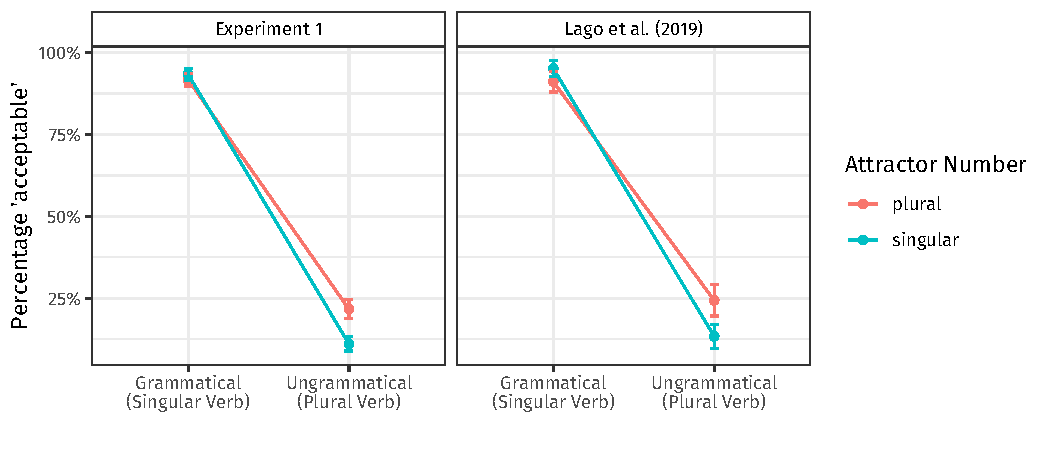
\includegraphics[width=\maxwidth]{figure/AverageResponses-1} 

}


\end{knitrout}

\caption{The average percentage of acceptable responses according to the experimental conditions in our study and \citet{LagoEtAl:2019}. Error bars signal standard errors calculated following \citet{Morey:2008,Cousineau:2005}.}
\label{fig:AverageResponses}
\end{figure}


Figure \ref{fig:ResponseModel} shows estimates and 95\% credible intervals of a Bayesian GLM with a probit link function. The main effect of grammaticality ($\hat{\beta}=3.04;$ $CI=[2.79; 3.29];$ $P(\beta<0)< .001$) indicates that, on average, participants were quite good at distinguishing between grammatical and ungrammatical sentences. Meanwhile, the negative interaction between grammaticality and attractor number ($\hat{\beta}=-0.72;$ $CI=[-1.00; -0.44];$ $P(\beta<0)> .999$) indicated a larger difference (positive) effect of plural attractors in ungrammatical conditions, and thus a number agreement attraction effect. There was weak evidence for a negative three-way interaction between the presence of ambiguity, ungrammaticality, and attractor number ($\hat{\beta}=-0.24;$ $CI=[-0.72; 0.25];$ $P(\beta<0)=    .83$), which was largely driven by differences in the effect of attractor number in \textit{grammatical conditions}, as the magnitude of the effect in the ungrammatical conditions was identical in both experiments (0.11).  
This is consistent with the estimates of the model based on ungrammatical sentences in Figure \ref{fig:ResponseModelUngram}, which show no indication of an interaction between ambiguity and the presence of a plural attractor (($\hat{\beta}=0.01;$ $CI=[-0.31; 0.33];$ $P(\beta<0)=    .46$). It also showed a main effect of plural attractor ($\hat{\beta}=0.46;$ $CI=[0.26; 0.65];$ $P(\beta<0)< .001$). Taken together, the coefficients indicated a substantial agreement attraction effect regardless of the presence of local ambiguity.  



\begin{figure}[hbt!]
\centering


\begin{knitrout}
\definecolor{shadecolor}{rgb}{0.969, 0.969, 0.969}\color{fgcolor}

{\centering 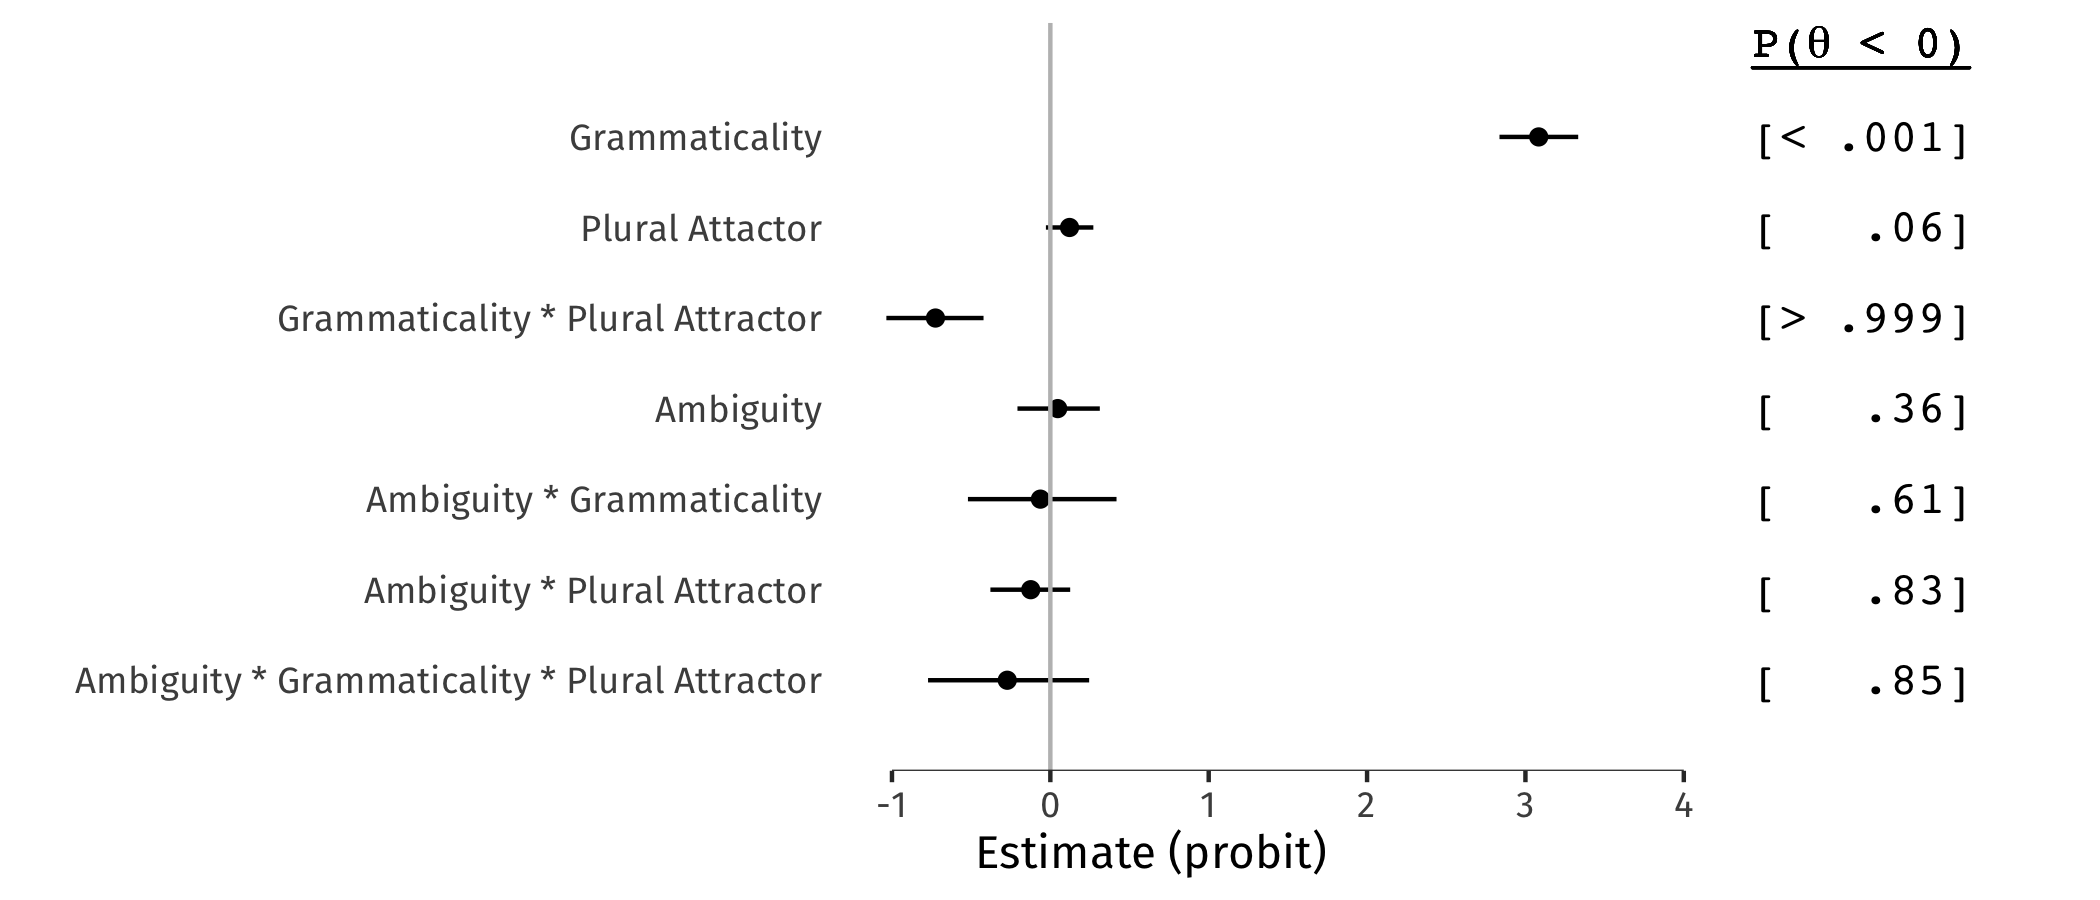
\includegraphics[width=\maxwidth]{figure/ResponseModel-1} 

}


\end{knitrout}

\caption{Estimates and 95\% credible intervals for the probit regression coefficients for the model of responses in our experiment and \citet{LagoEtAl:2019}.}
\label{fig:ResponseModel}
\end{figure}


\begin{figure}[hbt!]
\centering


\begin{knitrout}
\definecolor{shadecolor}{rgb}{0.969, 0.969, 0.969}\color{fgcolor}

{\centering 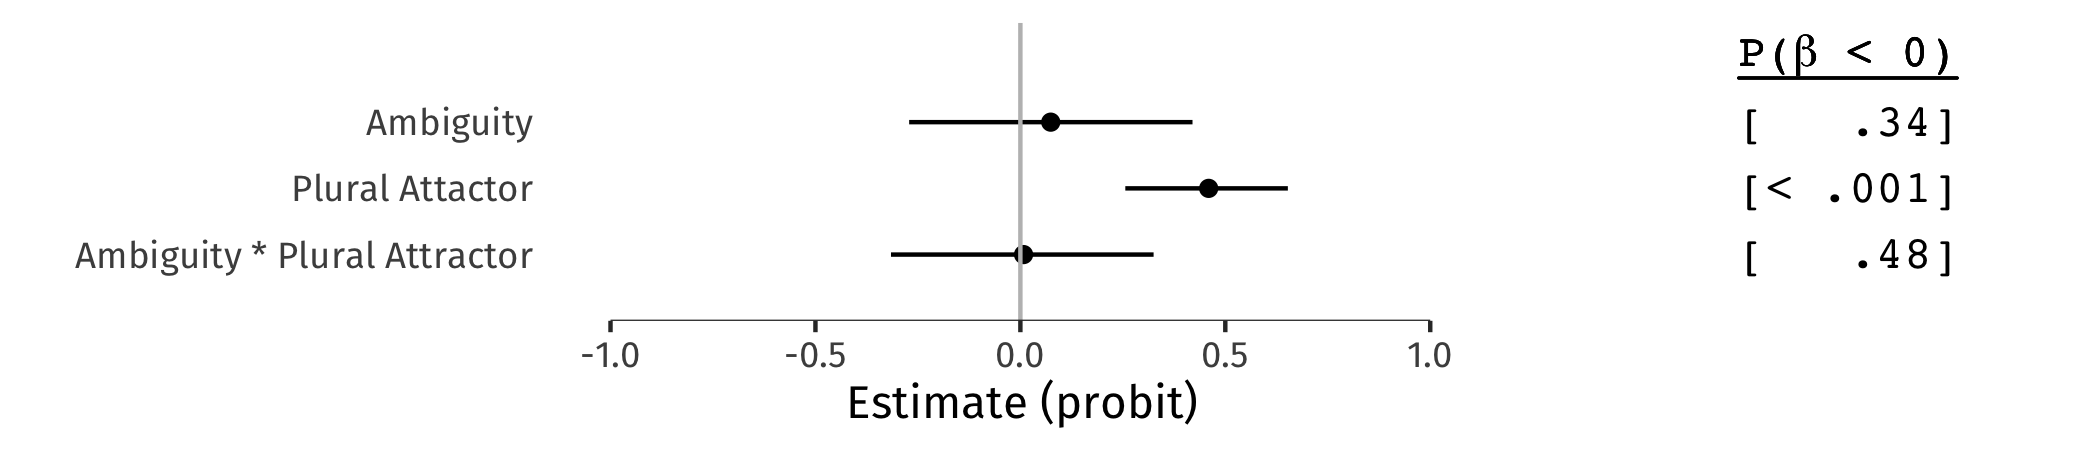
\includegraphics[width=\maxwidth]{figure/ResponseModelUngram-1} 

}


\end{knitrout}

\caption{Estimates and 95\% credible intervals for the probit regression coefficients for the model of responses to \protect{\textbf{ungrammatical sentences}} in our experiment and \citet{LagoEtAl:2019}.}
\label{fig:ResponseModelUngram}
\end{figure}


\section{Discussion \& Conclusion}

We re-examined the findings of \citet{LagoEtAl:2019} and investigated the contributution of a possible confound to their finding of an agreement attraction effect in genitive-possessive constructions in Turkish. Our main question was whether \citeauthor{LagoEtAl:2019}'s (\citeyear{LagoEtAl:2019}) findings can be explained by an alternative hypothesis: 
Because in their experimental sentences, all head nouns were locally ambiguous between the possessive and the accusative case (a non-subject case in Turkish), we hypothesized that this may have weakened the strength of association between the subject head noun and the subjecthood feature.
If Turkish agreement attraction effects in genitive-possessive structures resulted from this ambiguity, we expected the absence of agreement attraction effects when the case of the head noun was unambiguous.  

Our experimental findings were comparable to \citet{LagoEtAl:2019}: We observed that the presence of a plural attractor increased the rate of erroneous `acceptable' responses  
% increased the overall error rate
in ungrammatical sentences.
Importantly, we did not find an effect of case ambiguity: While our model based on all experimental conditions indicated a weak three-way interaction between ambiguity, grammaticality, and attractor number, a model based on ungrammatical sentences only demonstrated that this is due to a difference in acceptability rates in grammatical conditions. This model showed no evidence of an interaction between attractor number and ambiguity, indicating no evidence of a modulation of the effect size of the agreement attraction effect by the presence of a local case ambiguity. 
Although the $95\%$ credible interval for the interaction term was relatively wide, our findings indicate the presence of a substantial agreement attraction effect regardless of the presence of local ambiguity.
Thus, we successfully replicated the findings of \citet{LagoEtAl:2019} with disambiguated head nouns. 

Taken together, our results suggest (i) that agreement attraction effects in Turkish are not due to a reduced association between case-ambiguous nouns and the subjecthood features, and (ii) that local ambiguities, such as case syncretism, do not appear to play a role in agreement attraction. Participants do not appear to rely on form-related cues in their decision-making processes and instead use of abstract linguistic features as retrieval cues.

\section*{Abbreviations} %exclude


\textsc{dat} = dative, \textsc{gen} = genitive, \textsc{nmlz} = nominalizer, \textsc{pass} = passive, \textsc{pl} = plural, \textsc{poss} = possessive, \textsc{pst} = past, \textsc{sg} = singular, \textsc{when} = when. %exclude


\section*{Data Availability} %exclude


The data that support the findings of this study, the code, and the paper resources including \LaTeX{} and \texttt{Sweave} files are openly available in the anonimized github page at \url{https://anonymous.4open.science/r/tr_short_agreement_attraction-1365/}. %exclude


\section*{Authors' Contributions} %exclude


{\firstauthor} conceived the initial version of the presented idea. Both authors designed the the experiment together. 
{\firstauthor} wrote the stimuli and conducted the experiment. The statistical analysis was carried out by {\secondauthor}; {\firstauthor} prepared all summaries and plots. {\firstauthor} wrote the first draft of the manuscript and both authors edited it subsequently. 


%\printbibliography %for use with biblatex; comment out if you use natbib
%\bibliography{gp_short} %for use with natbib; comment out if you use biblatex, and change 'sample' by the name of your bib-file
\bibliographystyle{apacite}
\bibliography{gp_short.bib}

\end{document}
%%% Local Variables:
%%% mode: latex
%%% TeX-master: t
%%% TeX-engine: luatex
%%% End:
